\chapter{Introduction}\label{chapter:introduction}

\section{Topology in Antiquity}

\lipsum[1]
\begin{wrapfigure}{r}{0.5\textwidth}\label{fig:tetra}
  \setlength{\belowcaptionskip}{0em}
	\centering
	  \begin{tikzpicture}
      \node[anchor=south west,inner sep=0] (image) at (0,0) {\adjustbox{max width=\linewidth}{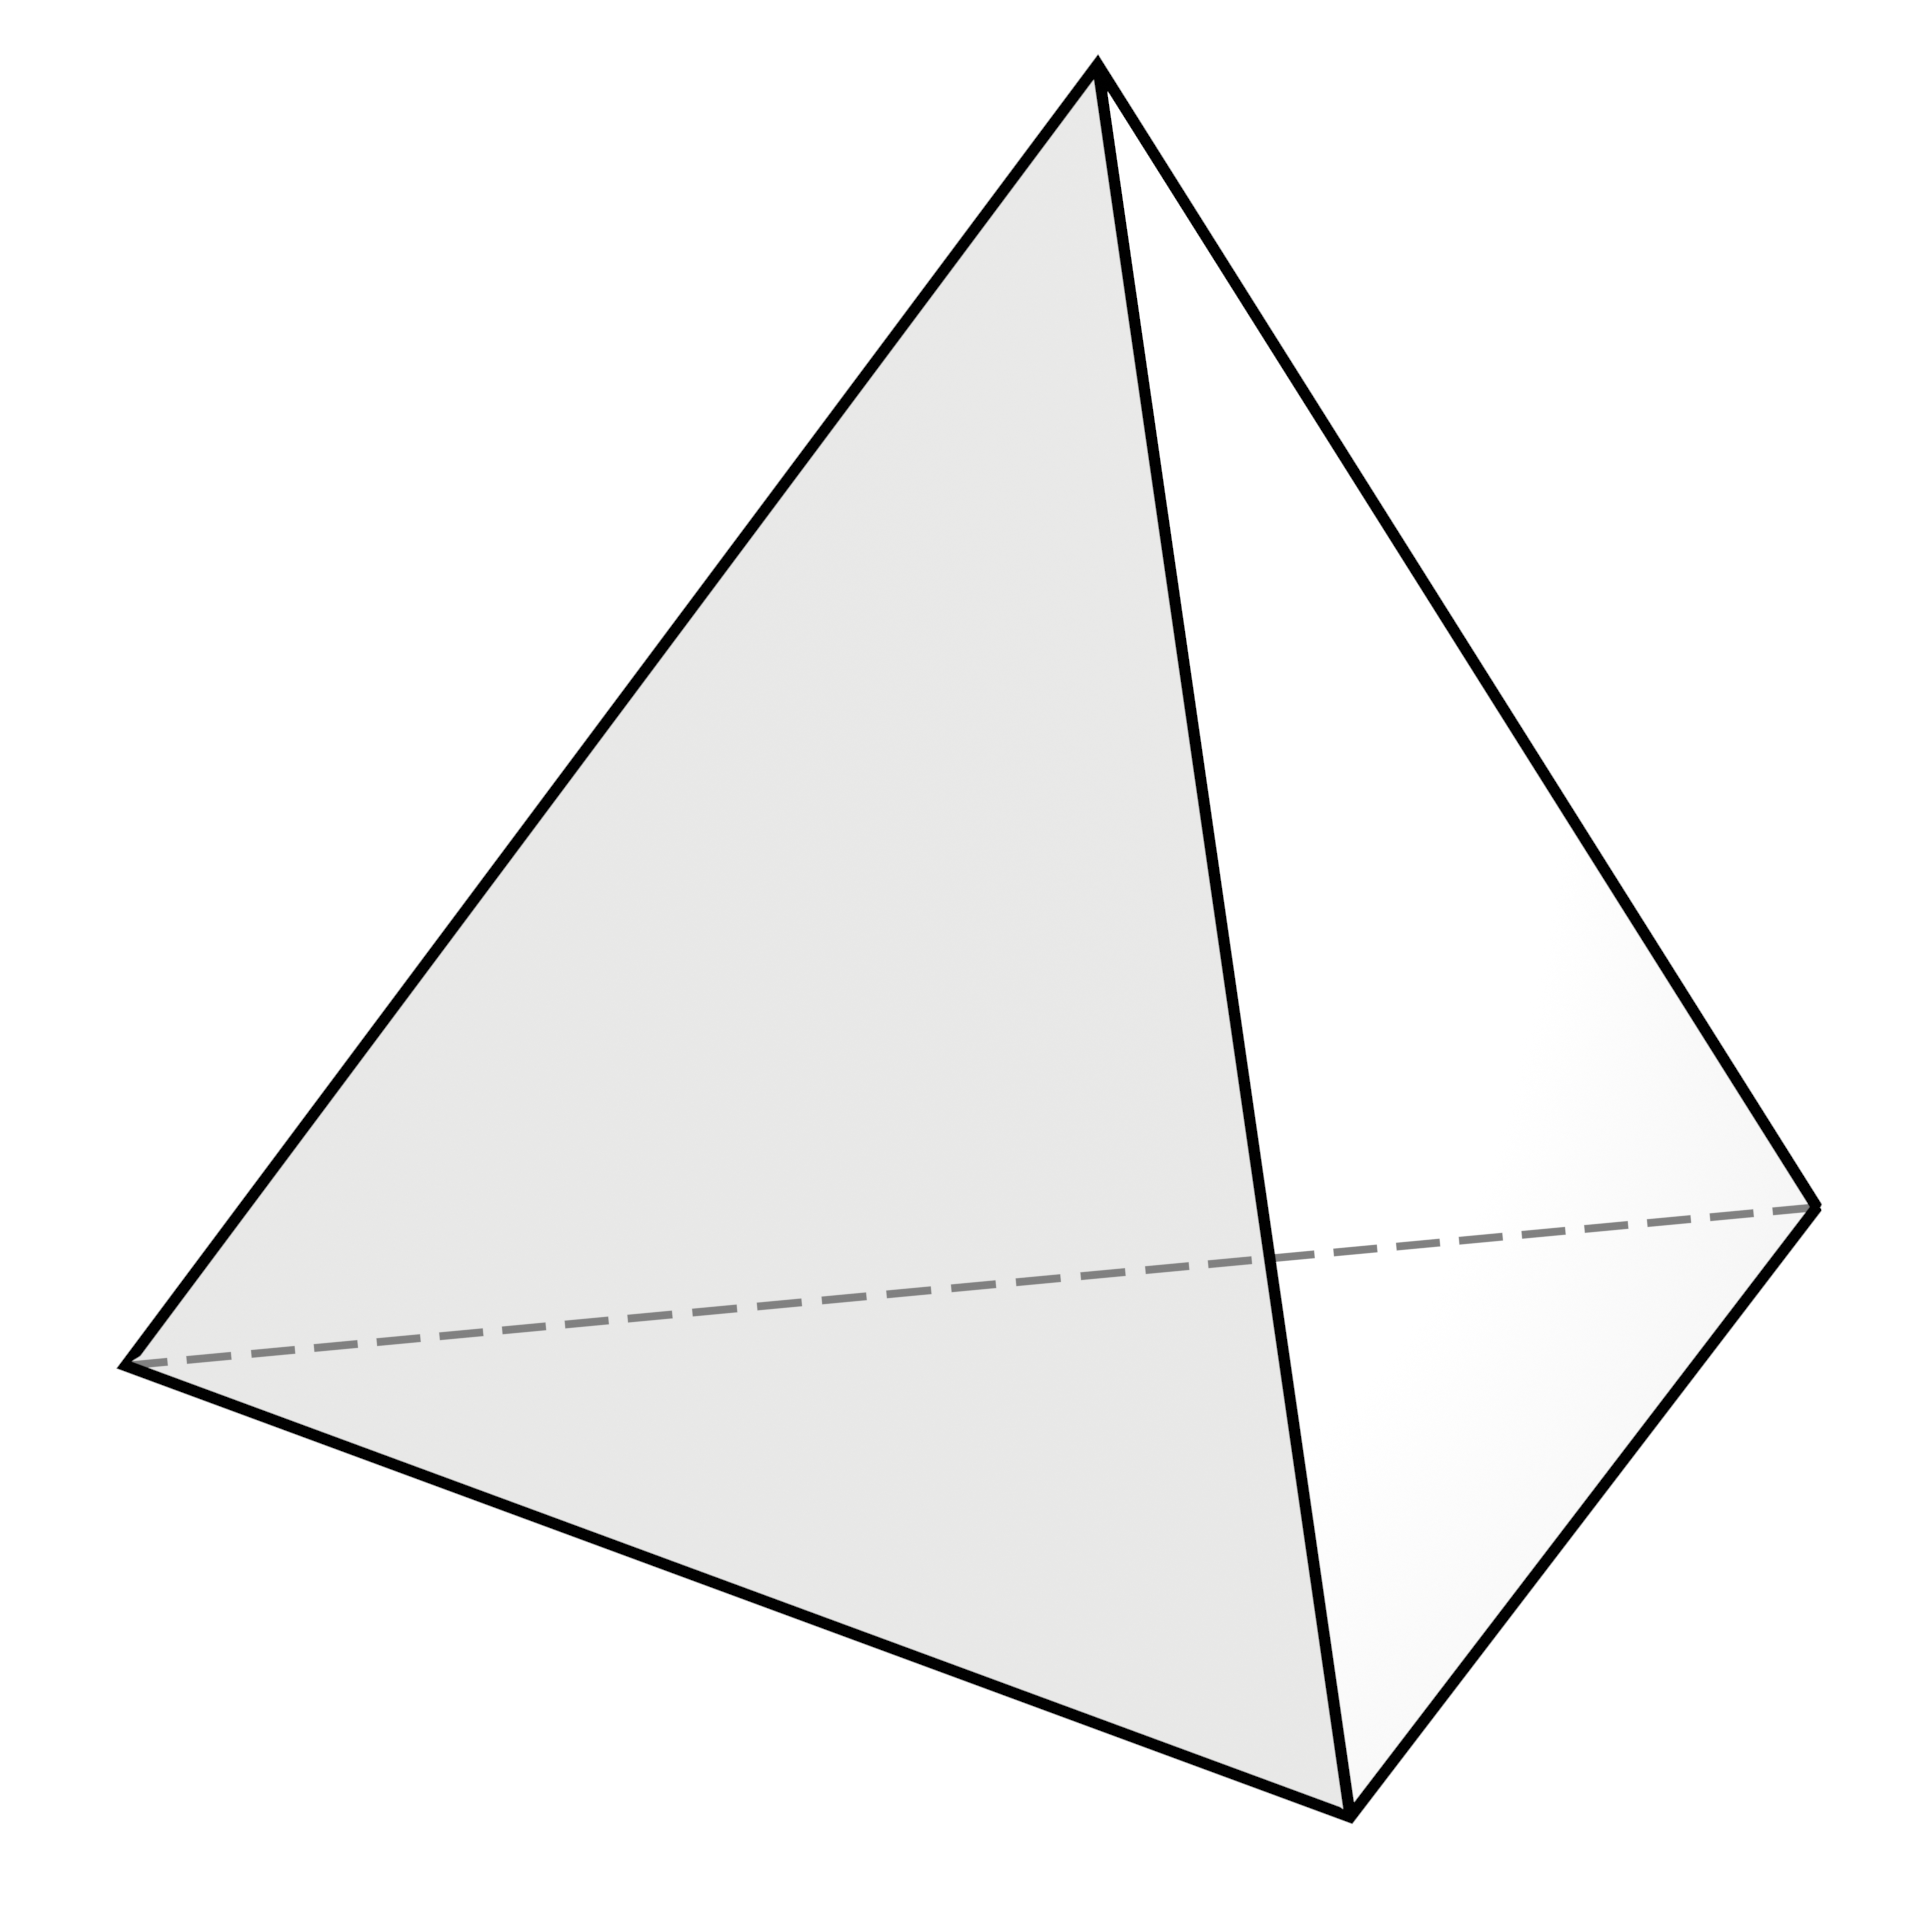
\includegraphics{graphics/tetra.png}}};

      \begin{scope}[x={(image.south east)},y={(image.north west)}]
          \draw[red,thick] (0.2,0.8) circle (0.05); 
          \node[blue] at (0.4,0.5) {$\displaystyle\int_X \omega\;dA$}; 
      \end{scope}
  \end{tikzpicture}
	\caption{A $3$-simplex}
\end{wrapfigure}

We can now introduce the main result of the paper:

\begin{definition}\label{def:pontryagin-og}
	Given a real vector bundle $E$ over $M$, it's \defn{$k$-th Pontryagin class}[Pontryagin class] $p_k(E)$ is defined as
	\[
		p_k(E) = (-1)^k c_{2k}(E\otimes \C) \in \H^{4k}(M; \Z),
	\]
	where $c_{2k}(E\otimes \C)$ denotes the $2k$-th Chern class of the complexification $E\otimes \C$.
\end{definition}
\lipsum[2]

\begin{wrapfigure}{l}{0.5\textwidth}\label{fig:cube-torus}
  \setlength{\belowcaptionskip}{0em}
	\centering
	  \begin{tikzpicture}
      \node[anchor=south west,inner sep=0] (image) at (0,0) {\adjustbox{max width=\linewidth}{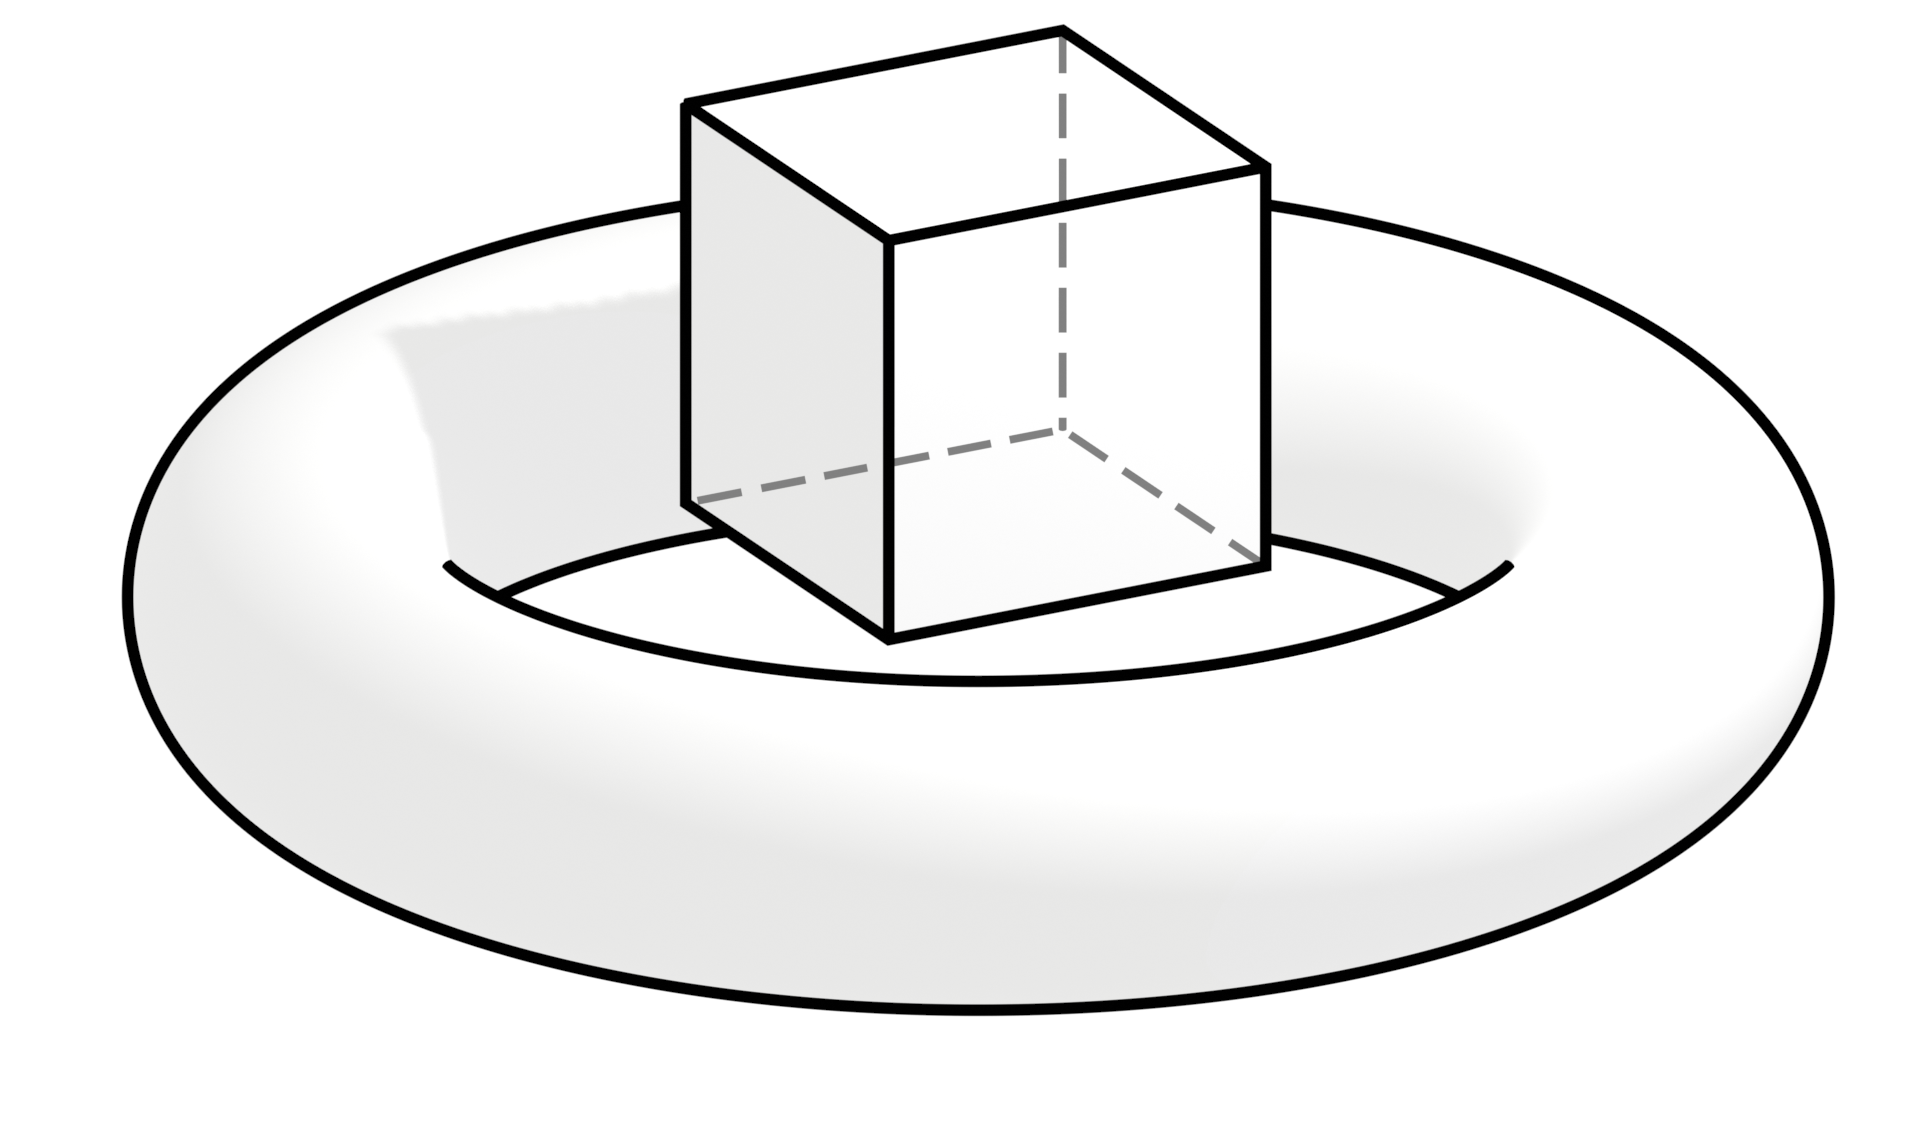
\includegraphics{graphics/cube-torus.png}}};
  \end{tikzpicture}
	\caption{A cube-torus}
\end{wrapfigure}

\lipsum[4-5]

\begin{wrapfigure}{r}{0.5\textwidth}\label{fig:principal_curvature}
  \setlength{\belowcaptionskip}{0em}
	\centering
	  \begin{tikzpicture}
      \node[anchor=south west,inner sep=0] (image) at (0,0) {\adjustbox{max width=\linewidth}{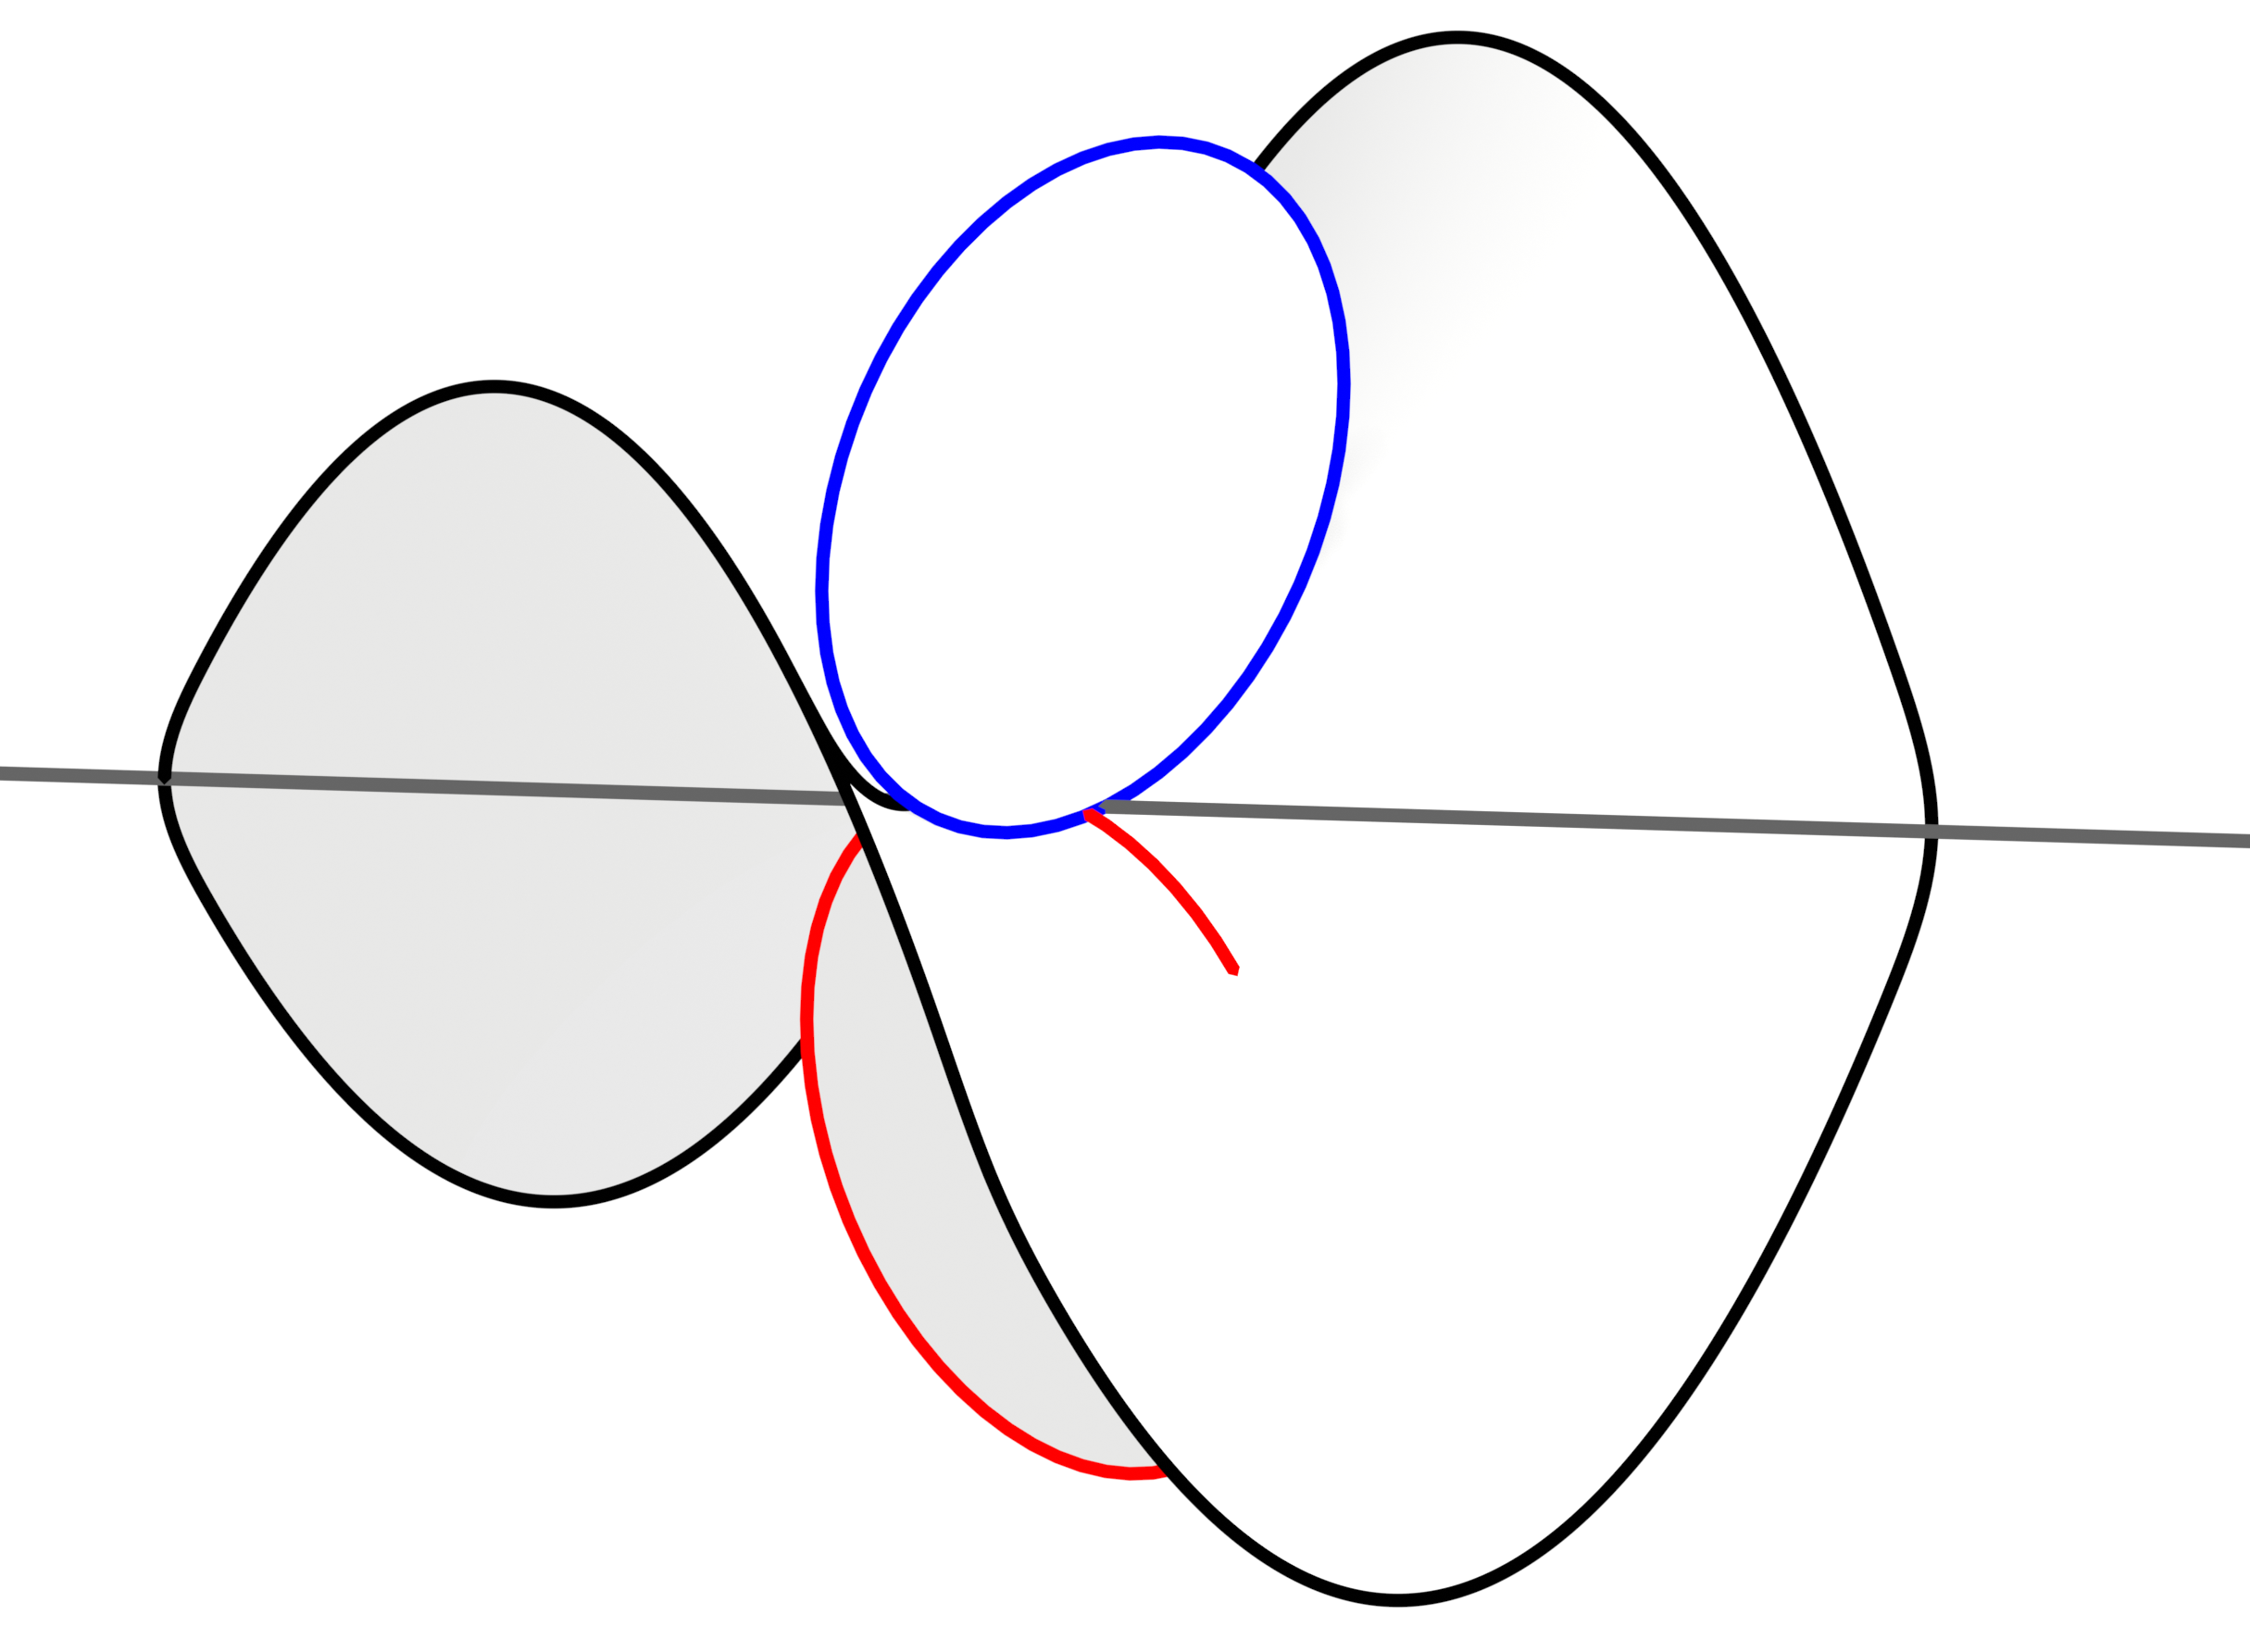
\includegraphics{graphics/principal_curvature.png}}};

      \begin{scope}[x={(image.south east)},y={(image.north west)}]
          \node[red] at (0.3,0.15) {$\kappa > 0$}; 
          \node[gray] at (0.65,0.55) {$\kappa = 0$}; 
          \node[blue] at (0.35,0.9) {$\kappa$ < 0}; 
      \end{scope}
  \end{tikzpicture}
	\caption{Curvatures for various normal planes}
\end{wrapfigure}

\lipsum[6]

\begin{figure}[ht]\label{fig:curvature}
  \setlength{\belowcaptionskip}{0em}
	\centering
	  \begin{tikzpicture}
      \node[anchor=south west,inner sep=0] (image) at (0,0) {\adjustbox{max width=\linewidth}{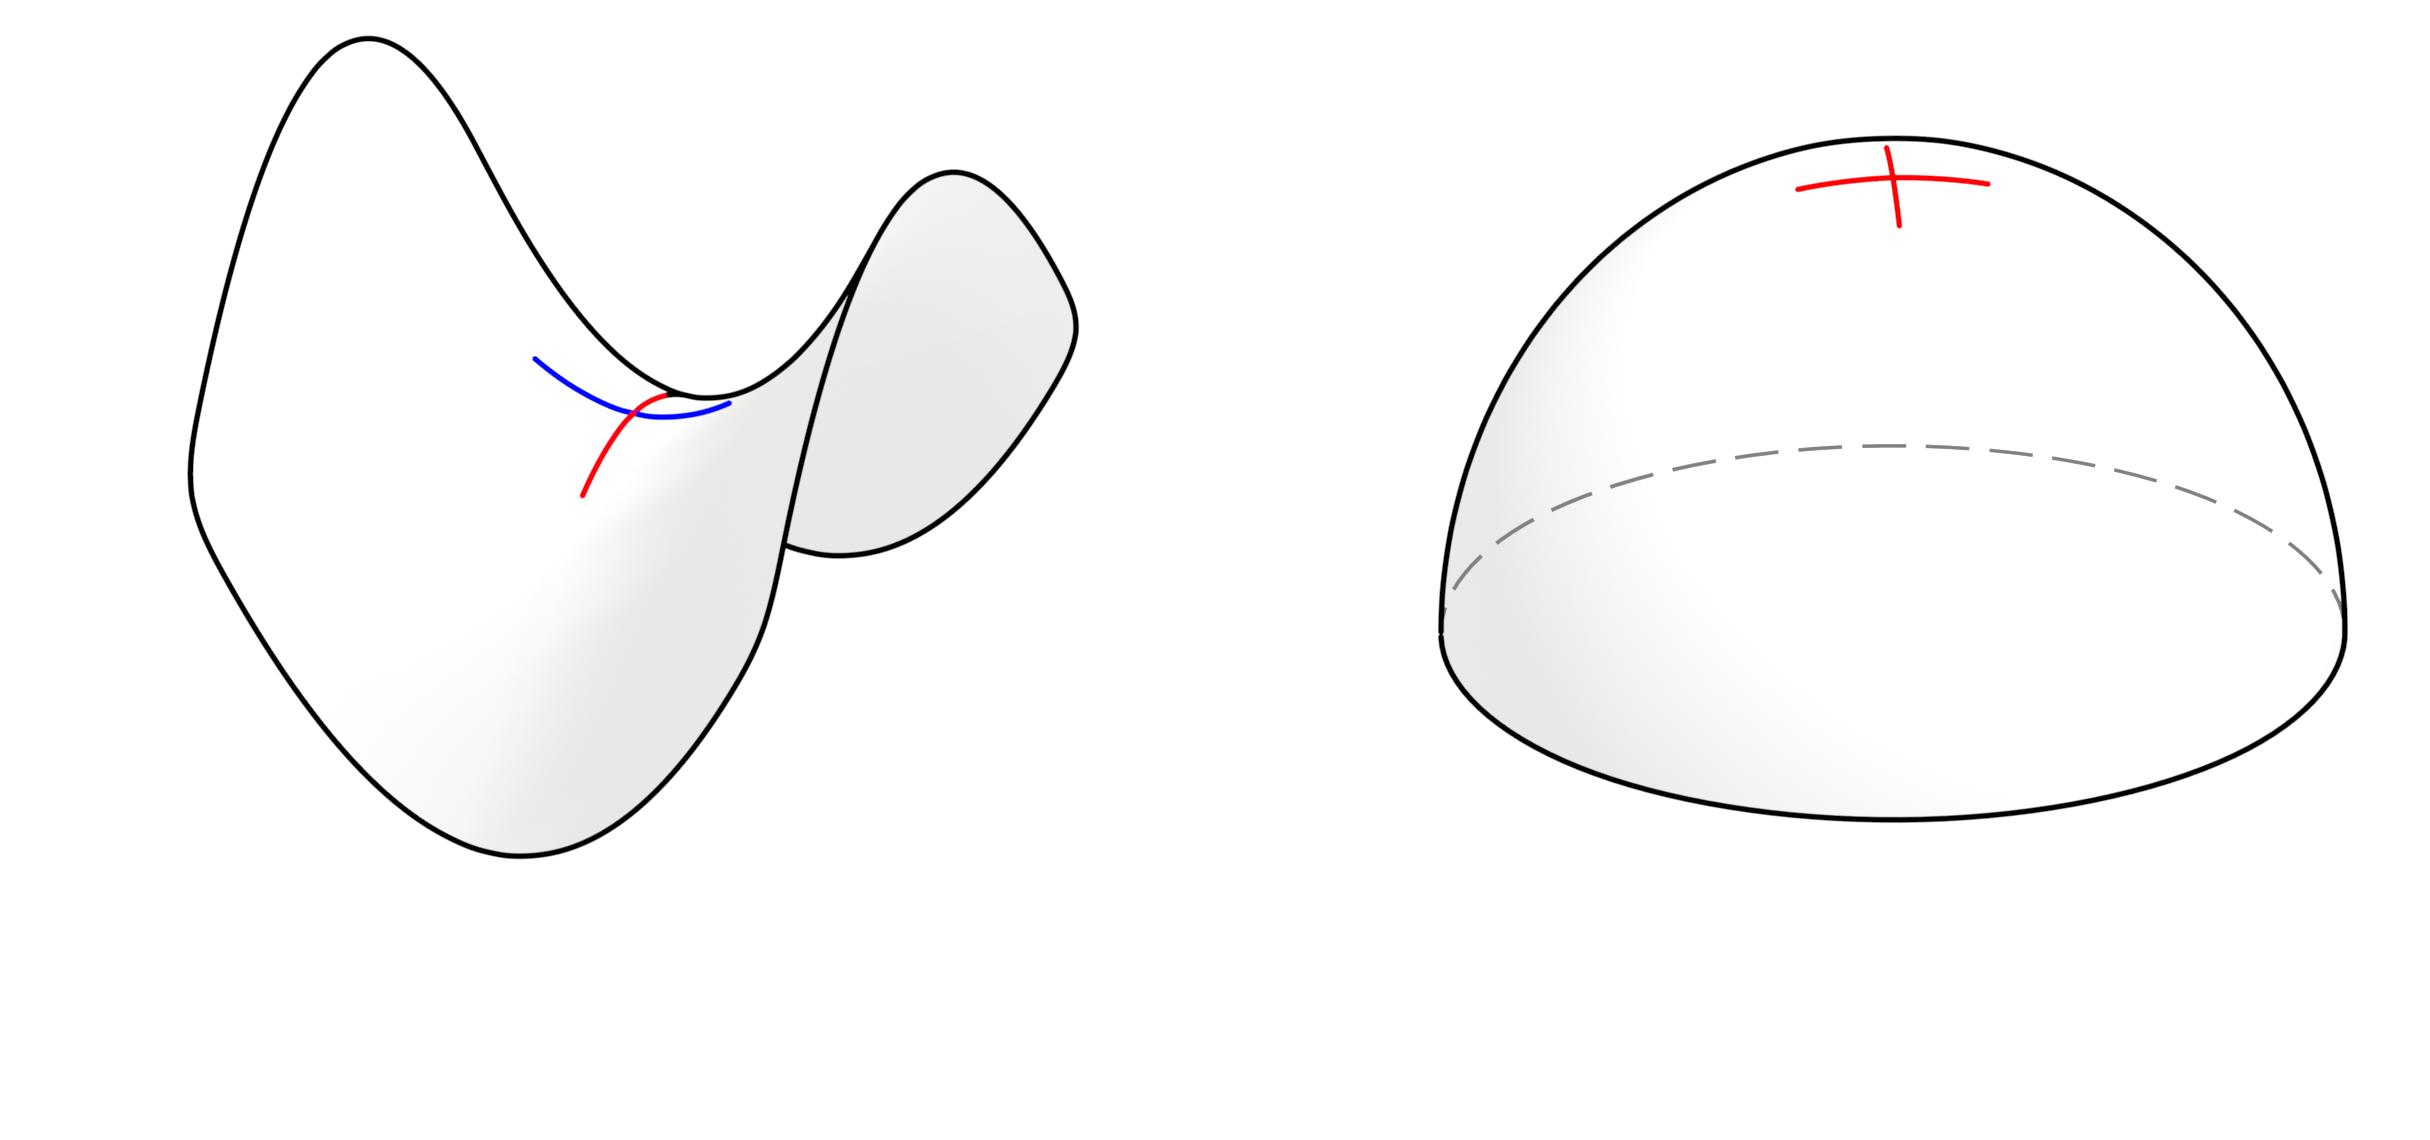
\includegraphics{graphics/curvature.png}}};

      \begin{scope}[x={(image.south east)},y={(image.north west)}]
          \node[red] at (0.23,0.53) {$\kappa_1$}; 
          \node[blue] at (0.2,0.7) {$\kappa_2$}; 

          \node[red] at (0.78,0.76) {$\kappa_1$}; 
          \node[red] at (0.72,0.82) {$\kappa_2$}; 
          \node[] at (0.2,0.1) {$K < 0$}; 
          \node[] at (0.75,0.1) {$K > 0$}; 
      \end{scope}
  \end{tikzpicture}
	\caption{Positive and negative curvature}
\end{figure}

\lipsum[6-8]
